\section{RESULTS}
In this section, we compare our results using PDT with those computed using
ONELD\cite{cepxs}. PDT is a three dimensional Parallel Deterministic Transport code developed at
Texas A\&M University while ONELD is a code that solves the  
equation (\ref{solved}) in one dimension using the cross sections generated by
CEPXS. ONELD always uses the full scattering order to solve photon-electron
transport problems. To compare the results produced by the two codes, we use 
equivalent angular discretization, Gauss-Legendre for ONELD, and 
Gauss-Legendre-Chebyshev (GLC) for our code. The GLC quadrature consists of 
a Gauss-Legendre quadrature for the polar angle and a Chebyshev quadrature 
for the azimuthal angle. The $n$-points Chebyshev quadrature uses $n$ points 
equally spaced between 0 and $2\pi$. When the solution is independent of the 
azimuthal angle, the GLC quadrature is equivalent to the one dimensional 
Gauss-Legendre quadrature. The results of ONELD gives only the average dose 
on a cell while the results of our code gives the dose at a given point. To 
compare the dose at any given point, we interpolate the values given by ONELD.

%\subsection{Water}
%Here, we use a $S_{12}$ quadrature. The medium is 5 cm thick and there is an 
%incoming flux of photons. The direction of the flux is chosen to be the most 
%normal direction of the quadrature and the value of the flux on the boundary is 1 
%$\frac{photon}{cm^2s}$. The source of photons has an energy of 20 MeV and we use 
%a cut-off energy of 0.01 MeV. Every particle that has an energy lower than 
%0.01 MeV is assumed to deposit all its energy without moving further.\\
%In the next table, we show the dose computed every centimeter using a
%different scattering \hbox{order :}
%\begin{table}[H]
%\begin{center}
%\caption{Dose in $\frac{MeV}{g}$ for different scattering orders}
%\begin{tabular}{|c|c|c|c|c|c|c|}
%\hline
%Position & ONELD & order = 13 & order = 11 & order = 9 & order = 7 & order = 5 \\
%\hline
%0 & 4.92645e-3 &  &  &  & 6.99349e-3 &  \\
%1 & 5.68274e-2 &  &  &  & 5.36101e-2 &  \\
%2 & 1.05076e-1 &  &  &  & 1.04073e-1 &  \\
%3 & 1.47528e-1 &  &  &  & 1.47958e-1 &  \\
%4 & 1.82864e-1 &  &  &  & 1.81629e-1 &  \\
%5 & 1.85907e-1 &  &  &  & 1.56533e-1 &  \\
%\hline
%\end{tabular}
%\end{center}
%\end{table}     

\subsection{Aluminium}
The medium is 5 cm thick and made of aluminium. We use a $S_{12}$ quadrature. 
There is an incoming flux of photons of 1 $\frac{photon}{cm^2}$. The direction
of the incoming flux is 
chosen to be the most normal direction of the quadrature. The source of photons has an 
energy of 20 MeV and we use a cut-off energy of 0.01 MeV. Every particle that has 
an energy lower than 0.01 MeV is assumed to deposit all its energy without moving 
further.\\
In the following table, we vary the number of moments and we show the dose computed 
every centimeter using different scattering orders. Notice that the order
thirteen is the full order, i.e. the number of moments equals the number of directions.
\begin{table}[H]
\begin{center}
\caption{\bf{Dose in $\frac{MeV}{g}$ for different scattering orders}}
\begin{tabular}{|c|c|c|c|c|c|c|}
\hline
Position (cm) & ONELD & \multicolumn{5}{c|}{PDT} \\
\hline
   & & order = 13 & order = 11 & order = 9 & order = 7 & order = 5 \\
\hline
0 & 0.015003 & 0.0146404 & 0.0146402 & 0.0141156 & 0.0166718 & 0.0087276 \\
1 & 0.169908 & 0.1697907 & 0.1697890 & 0.1698012 & 0.1695422 & 0.1728969 \\
2 & 0.275425 & 0.2752749 & 0.2752729 & 0.2753298 & 0.2742052 & 0.2775113 \\
3 & 0.316307 & 0.3161310 & 0.3161307 & 0.3165279 & 0.3145572 & 0.3199176 \\
4 & 0.312283 & 0.3120572 & 0.3120566 & 0.3125514 & 0.3104412 & 0.3153226 \\
5 & 0.233048 & 0.2087631 & 0.2087634 & 0.2094064 & 0.2061794 & 0.2154810 \\
\hline
\end{tabular}
\end{center}
\end{table}     
The relative error are :
\begin{table}[H]
\begin{center}
\caption{\bf{Relative error in percentage for different scattering orders}}
\begin{tabular}{|c|c|c|c|c|c|}
\hline
Position (cm) & \multicolumn{5}{c|} {PDT}\\
\hline
& order = 13 & order = 11 & order = 9 & order = 7 & order = 5 \\
\hline
0 & 2.41\% & 2.41\% & 5.91\% & 11.1\% & 41.8\% \\
1 & 0.069\% & 0.07\% & 0.062\% & 0.21\% & 1.79\% \\
2 & 0.054\% & 0.055\% & 0.035\% & 0.44\% & 0.76\% \\
3 & 0.056\% & 0.056\% & 0.070\% & 0.55\% & 1.14\% \\
4 & 0.072\% & 0.072\% & 0.085\% & 0.59\% & 0.97\% \\
5 & 10.42\% & 10.42\% & 10.14\% & 11.53\% & 7.53\% \\
\hline
\end{tabular}
\end{center}
\end{table}     
The agreement between ONELD and our code using the full order is excellent.
The differences on the edges of the domain are larger, due to the fact that
the dose varies quickly near the border. Because of this, the interpolation 
used to find the value at a given point by ONELD is less precise.\\ 
We see that if we discard the results on the edges of the domain, the results 
obtained by using a $P_5$ order for the scattering are very close to the ones 
using the full order in the scattering cross-section expansion. The reason is 
that the high order flux moments are very small compared to the low order flux
moments (see Figure \ref{test1} to Figure \ref{test6}). In the following figures, the 
abscissa is the distance in centimeters and the ordinate is the value of the 
flux in $\frac{particles}{cm^2s}$.
\begin{figure}[H]
\begin{minipage}[b]{0.42\linewidth}
\centering
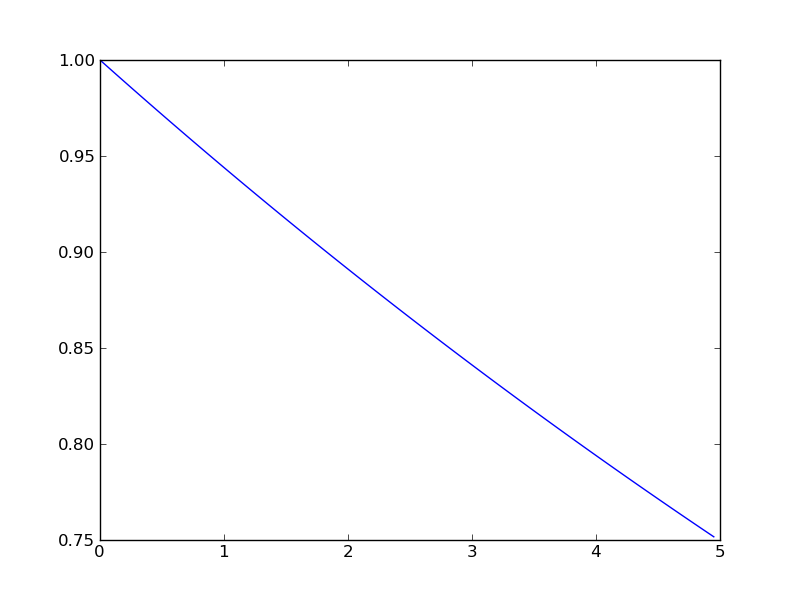
\includegraphics[width=\linewidth]{./images/al/group_0_moment_0}
\caption{\bf{Scalar flux in the first photon group}}
\label{test1}
\end{minipage}
\hspace{0.5cm}
\begin{minipage}[b]{0.42\linewidth}
\centering
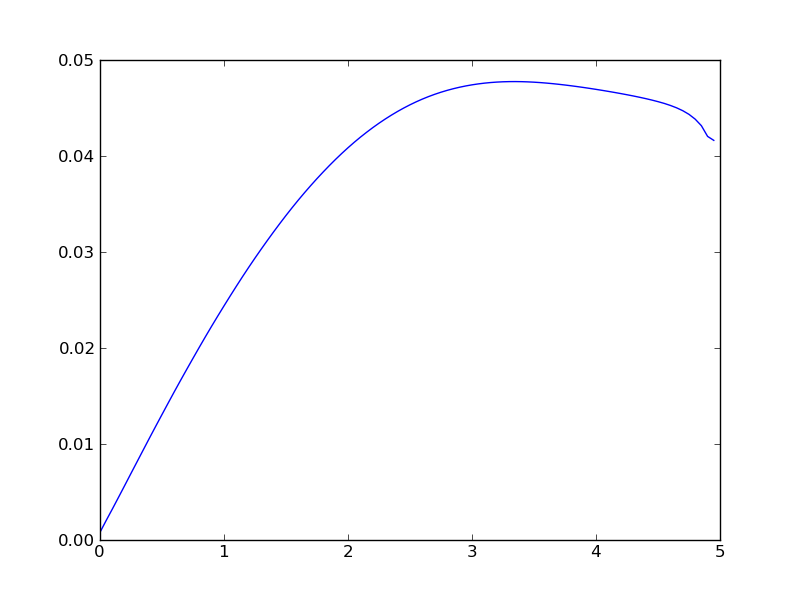
\includegraphics[width=\linewidth]{./images/al/group_39_moment_0}
\caption{\bf{Scalar flux in the last electron group}}
\label{test2}
\end{minipage}
\end{figure}

\begin{figure}[H]
\begin{minipage}[b]{0.42\linewidth}
\centering
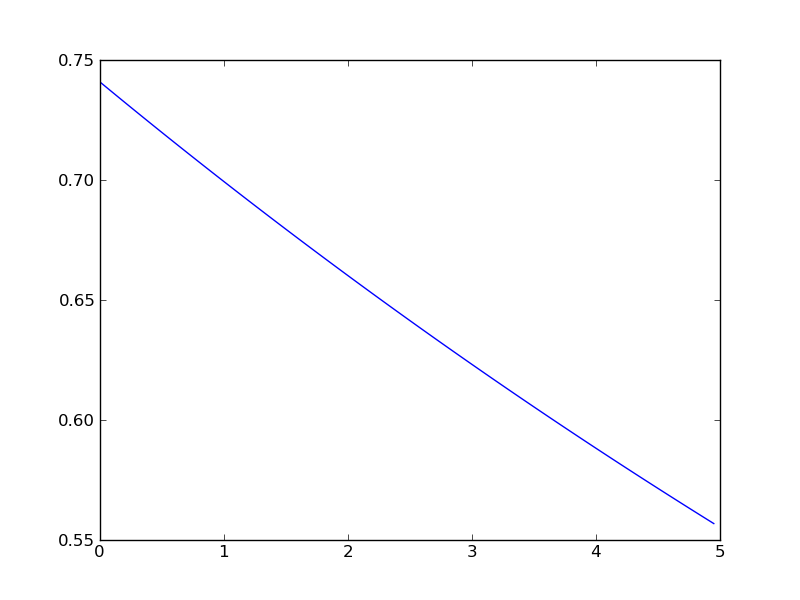
\includegraphics[width=\linewidth]{./images/al/group_0_moment_30}
\caption{\bf{Moment $\mathbf{P_5^0}$ of the flux in the first photon group}}
\label{test3}
\end{minipage}
\hspace{0.5cm}
\begin{minipage}[b]{0.42\linewidth}
\centering
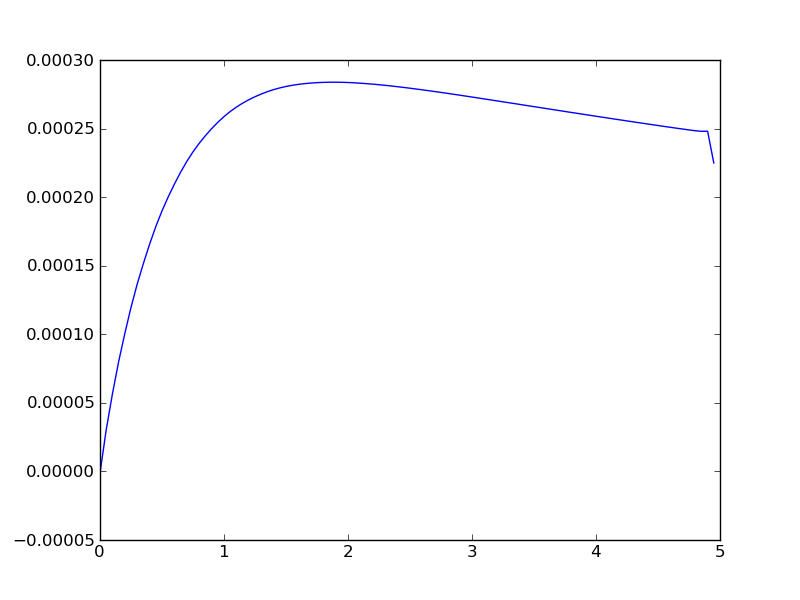
\includegraphics[width=\linewidth]{./images/al/group_39_moment_30}
\caption{\bf{Moment $\mathbf{P_5^0}$ of the flux in the last electron group}}
\label{test4}
\end{minipage}
\end{figure}

\begin{figure}[H]
\begin{minipage}[b]{0.42\linewidth}
\centering
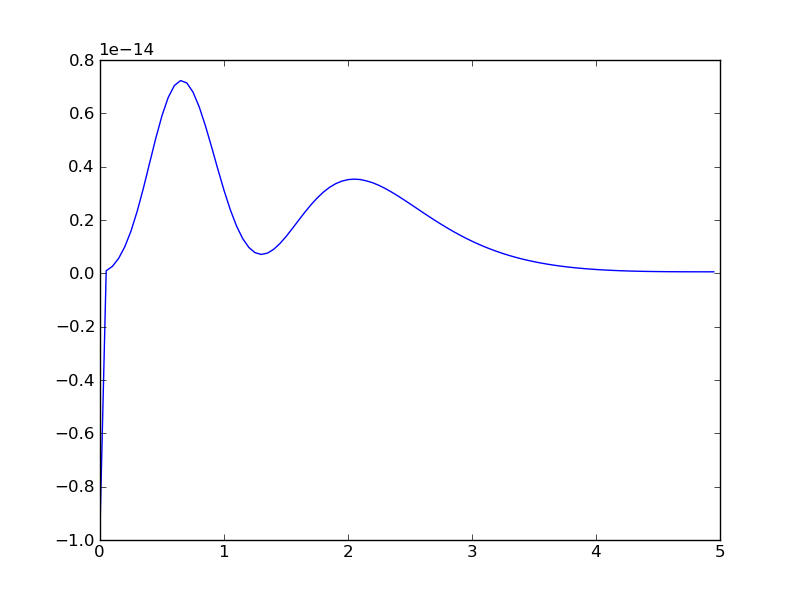
\includegraphics[width=\linewidth]{./images/al/group_0_moment_142}
\caption{\bf{Moment $\mathbf{P_{11}^0}$ of the flux in the first photon group}}
\label{test5}
\end{minipage}
\hspace{0.5cm}
\begin{minipage}[b]{0.42\linewidth}
\centering
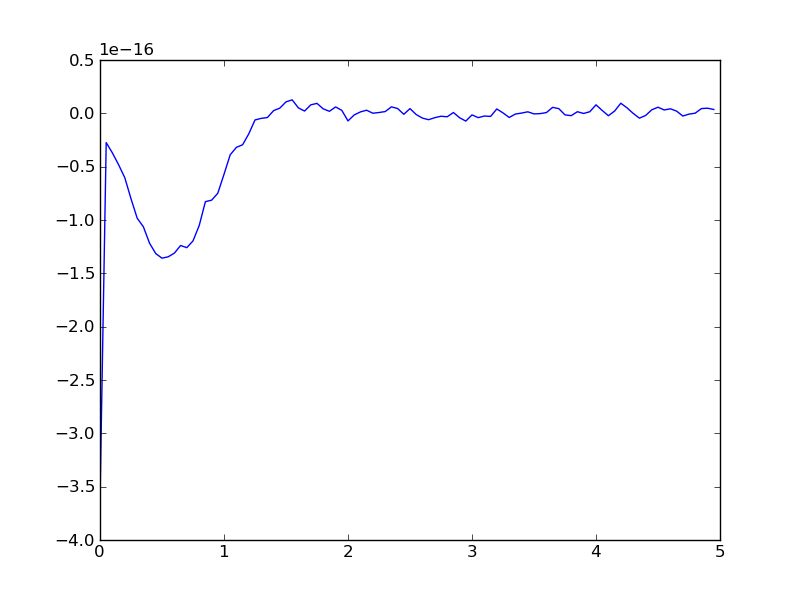
\includegraphics[width=\linewidth]{./images/al/group_39_moment_142}
\caption{\bf{Moment $\mathbf{P_{11}^0}$ of the flux in the last electron group}}
\label{test6}
\end{minipage}
\end{figure}

\subsection{Gold}
The setup of this problem is the same as for the previous simulations but the
medium considered here is gold. In the next table, we provide the dose
computed every centimeter using different scattering orders :
\begin{table}[H]
\begin{center}
\caption{\bf{Dose in $\frac{\mathbf{MeV}}{\mathbf{g}}$ for different scattering orders}}
\begin{tabular}{|c|c|c|c|c|c|}
\hline
Position (cm) & ONELD & \multicolumn{4}{c|}{PDT} \\
\hline
 &  &  order = 11 & order = 9 & order = 7 & order = 5 \\
\hline
0 & 0.11675 & 0.097168 & 0.097155 & 0.097073 & 0.097326 \\
1 & 0.41799 & 0.420905 & 0.420871 & 0.420988 & 0.421102 \\
2 & 0.16284 & 0.164953 & 0.164946 & 0.165017 & 0.164605 \\
3 & 0.06407 & 0.065297 & 0.065300 & 0.065292 & 0.065214 \\
4 & 0.02566 & 0.026303 & 0.026304 & 0.026295 & 0.026318 \\
5 & 0.00847 & 0.006082 & 0.006083 & 0.006075 & 0.006112 \\
\hline
\end{tabular}
\end{center}
\end{table}                
The relative errors are given in the next table :
\begin{table}[H]
\begin{center}
\caption{\bf{Relative error in percentage for different scattering orders}}
\begin{tabular}{|c|c|c|c|c|}
\hline
Position (cm) & \multicolumn{4}{c|}{PDT}\\
\hline
 & order = 11 & order = 9 & order = 7 & order = 5 \\
\hline
0 & 16.77\% & 16.78\% & 16.85\% & 16.64\% \\
1 & 0.70\% & 0.70\% & 0.72\% & 0.74\% \\
2 & 1.30\% & 1.29\% & 1.02\% & 1.08\% \\
3 & 1.92\% & 1.92\% & 1.91\% & 1.79\% \\
4 & 2.51\% & 2.51\% & 2.47\% & 2.56\% \\
5 & 28.19\% & 28.18\% & 28.28\% & 27.84\% \\
\hline
\end{tabular}
\end{center}
\end{table}     
We can see that there is no need to use the full order to solve the problem.
The differences between the order five and order eleven are small. For this reason,
we expect the results of the order eleven to be very close from the ones of
order eleven. The difference between the order eleven and ONELD
is about 2\% in the middle of the domain while the difference is larger on the
boundary of the domain due to the interpolation of the ONELD results.

